\chapter{Preliminaries}\label{chapter:preliminaries}
This chapter introduces the mathematical structures that underlie the temporal component of our normative framework, together with the basic models used to represent system executions. We focus on representations that allow timed constraints to be stated, combined, and analyzed symbolically, without committing to a particular execution or monitoring model. In parallel, we introduce trace-based word models that serve as the semantic carriers for observed behavior and interaction. The material in this chapter is intentionally elementary and self contained. Its purpose is not to introduce new logical operators, but to establish precise domains for manipulating time ranges and executions algebraically, which will later be embedded into normative specifications and monitoring constructions.
\section{Interval Set over Integers}
Timed constraints in normative systems are rarely punctual. Obligations and prohibitions typically apply over contiguous or fragmented time ranges, and reasoning directly over individual time points leads to unnecessary blow up. For this reason, we adopt sets of intervals as our basic representation of temporal constraints. Interval sets provide a compact and canonical way to capture possibly discontinuous time ranges, while still supporting precise arithmetic operations such as intersection, union, and difference. Before introducing interval sets and their algebra, we first fix the underlying numerical domain on which these intervals are defined.
\subsection{Natural Numbers and Extended Natural Numbers}

Let  $\mathbb{N}$ denote the set of all positive integers including zero, i.e.\ \( \mathbb{N}:= \{ 0, 1, 2, 3, \dots \} \) and let \emph{less} ($<$) and  \emph{less or equal} ($\leq$) denote the usual order relations on $\mathbb{N}$.
%
We extend \(\mathbb{N}\) by adding the element \(\infty\), denoting infinity, forming the set of extended  natural numbers: % ML@KK: define macros for example for \mathbb{N}^\infty 
\( \mathbb{N}^\infty = \mathbb{N} \cup \{\infty\} \).
We define  the order relations for  $\mathbb{N}^\infty$ : $<_\infty$ and  $\leq_\infty$:

            \[
           \text{For } n,m \in \mathbb{N}^\infty, n <_\infty m \text{ if and only if }
            \begin{cases} 
                n \in \mathbb{N} \text{ and } m \in \mathbb{N} \text{ and } n < m,\\
                n \in \mathbb{N} \text{ and } m = \infty.
            \end{cases}
            \]
            \[
             \text{For } n,m \in \mathbb{N}^\infty,n \leq_\infty m \text{ if and only if }
            \begin{cases} 
                n \in \mathbb{N} \text{ and } m \in \mathbb{N} \text{ and } n \leq m,\\
                n \in \mathbb{N} \text{ and } m = \infty,\\
                n = \infty \text{ and } m = \infty.
            \end{cases}
            \]
\subsection{Intervals}


\begin{definition}[Interval]
A \emph{non-empty interval} is a pair $[\tmin,\tmax]$ with $\tmin \in \mathbb{N}$, $\tmax \in \mathbb{N}^\infty$, and $\tmin \leq_\infty \tmax$. The \emph{empty interval}, written $\varnothing$, contains no elements.
The set of all valid intervals is
%\[
defined as $
\mathbb{I} := \{[\tmin,\tmax] \mid \tmin \leq_\infty \tmax\} \cup \{\varnothing\}.
$
%\]
For $n\in\mathbb{N}$, we write $n\in[\tmin,\tmax]$ iff $\tmin \leq_\infty n \leq_\infty \tmax$. 
 \end{definition}

 Informally, a non-empty interval $[\tmin,\tmax]$  \emph{represents} a contiguous set of numbers, that is:  $\{n \mid n\in[\tmin,\tmax]\}$, and the empty interval $\varnothing$ represents the empty set of natural numbers.
The \emph{size} of an interval $I$, written $\size{I}$, relates to the cardinality of the set that it represents. Thus, the size for $\varnothing$ is zero and for valid non-empty intervals:
\[
\size{[a,b]} :=
\begin{cases}
b-a-1 & \text{if } b\!\in\!\mathbb{N},\\
\infty & \text{if } b=\infty.
\end{cases}
\]

  \begin{example} 
  Consider the following examples of intervals:
\begin{itemize}
    \item If \(\tmin := 2\) and \(\tmax := 5\), then \(I := [2, 5] \text{ represents } \{ 2, 3, 4, 5 \}\).
    \item If \(\tmin := 3\) and \(\tmax := \infty\), then \(I := [3, \infty] \text{ represents }\{ t \in \mathbb{N} \mid t \geq 3 \}\).
    \item If \(\tmin := 3\) and \(\tmax := 3\), then \(I := [3, 3] \text{ represents } \{ 3\}\).
     \item If \(\tmin := 3\) and \(\tmax := 0\), then $I:=[3,0]$ is not a valid interval.
\\

     We transform the timed constraints from the  use case to intervals:
     \begin{enumerate}
         \item Let $I_1:=[9,16]$ represent the timed constraint between 9:00 and 16:00 from the Delivery Clause (Table~\ref{tab:contract}).
         \item Let $I_2:=[8, 24]$ represent the constraint between 8:00 and 24 from the Maintenance Announcement (Table~\ref{tab:ma}).
         \item Let $I_3:=[10,14]$ represent the constraint between 10:00 and 14:00 from the Safety regulation (Table \ref{tab:contract}).
     \end{enumerate}
\end{itemize}
\end{example}


\subsection{Allen's Algebra and Unifiability}


Allen's algebra \cite{allen1983maintaining} consists of 13 exhaustive and mutually exclusive relations between \textit{abstract}\footnote{Not inherently tied to a specific numerical domain.} pairs of intervals. To provide an intuition, in Fig.~\ref{fig:ia} we give a visual interpretation of these relations. The different cases are based on the relative comparison of the start and end points of the intervals. In Table \ref{tab:IAdesc} we specify the constraints associated with each case for the domain of intervals $\mathbb{I}$ defined on natural numbers.


\begin{figure}[h]
    \begin{subfigure}{0.22\textwidth}
        \centering
          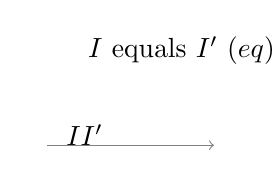
\begin{tikzpicture}[scale=0.5, yscale=0.80]
            \draw[->,gray] (-0.5,0) node[left] {} -- (3.75,0);
            \drawinterval{.5}{1.7}{2.5}{1.7}{$I$}
            \drawinterval{.5}{.7}{2.5}{.7}{$I'$}
            \node[] at (2,3) {$I$ equals $I'$ ($eq$)};
        \end{tikzpicture}
        %\caption*{$I$ equals $I'$ ($eq$)}
        \label{subfig:ia:eg}
    \end{subfigure}
    \hfill
    \begin{subfigure}{0.19\textwidth}
        \centering
          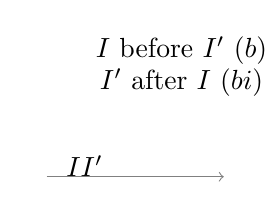
\begin{tikzpicture}[scale=0.5, yscale=0.80]
            \draw[->,gray] (-0.5,0) node[left] {} -- (4,0);
            \drawinterval{0}{1.7}{1.4}{1.7}{$I$}
            \drawinterval{1.9}{.7}{3.35}{.7}{$I'$}
            \node[] at (2,4) {$I$ before $I'$ ($b$)};
            \node[] at (2,3) {$I'$ after $I$ ($bi$)};
        \end{tikzpicture}
        \label{subfig:ia:b}
    \end{subfigure}
    \hfill 
    \begin{subfigure}{0.22\textwidth}
        \centering
          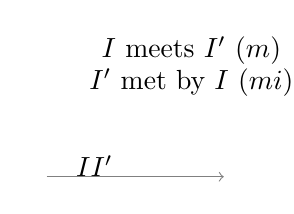
\begin{tikzpicture}[scale=0.5, yscale=0.80]
            \draw[->,gray] (-0.75,0) node[left] {} -- (3.75,0);
            \drawinterval{0}{1.7}{1.5}{1.7}{$I$}
            \drawinterval{1.5}{.7}{3}{.7}{$I'$}
            \node[] at (2,4) {$I$ meets $I'$ ($m$)};
            \node[] at (2,3) {$I'$ met by $I$ ($mi$)};
        \end{tikzpicture}
        \label{subfig:ia:m}
    \end{subfigure}
    \hfill 
    \begin{subfigure}{0.22\textwidth}
        \centering
          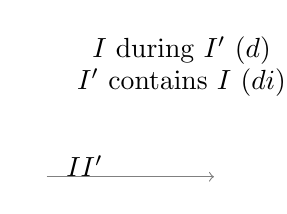
\begin{tikzpicture}[scale=0.5, yscale=0.80]
            \draw[->,gray] (-0.5,0) node[left] {} -- (3.75,0);
            \drawinterval{0.5}{1.7}{2.5}{1.7}{$I$}
            \drawinterval{0}{.7}{3.1}{.7}{$I'$}
            \node[] at (2,4) {$I$ during $I'$ ($d$)};
            \node[] at (2,3) {$I'$ contains $I$ ($di$)};
        \end{tikzpicture}
        \label{subfig:ia:d}
    \end{subfigure}
    \vspace{0.05cm}
    \quad
    \hfill 
    \begin{subfigure}{0.23\textwidth}
        %\caption*{$I$ starts $I'$ ($s$)\\ $I'$ started by $I$ ($si$)}
        \centering
          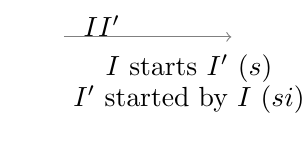
\begin{tikzpicture}[scale=0.5, yscale=0.80]
            \draw[->,gray] (-0.5,0) node[left] {} -- (3.75,0);
            \drawinterval{0}{1.7}{1.15}{1.7}{$I$}
            \drawinterval{0}{.7}{3.1}{.7}{$I'$}
            \node[] at (1.75,-1) {$I$ starts $I'$ ($s$)};
            \node[] at (1.75,-2) {$I'$ started by $I$ ($si$)};            
        \end{tikzpicture}
        \label{subfig:ia:s}
    \end{subfigure}
    \hfill
    \begin{subfigure}{0.22\textwidth}
        %\caption*{$I$ overlaps $I'$ ($o$)\\ $I'$ overlapped by $I$ ($oi$)}
        \centering
          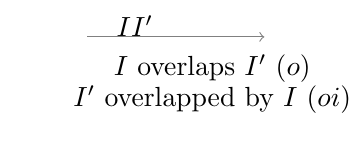
\begin{tikzpicture}[scale=0.5, yscale=0.80]
            \draw[->,gray] (-0.75,0) node[left] {} -- (3.75,0);
            \drawinterval{0}{1.7}{1.5}{1.7}{$I$}
            \drawinterval{1.2}{.7}{2.8}{.7}{$I'$}
            \node[] at (1.5,-1) {$I$ overlaps $I'$ ($o$)};
            \node[] at (1.5,-2) {$I'$ overlapped by $I$ ($oi$)};
        \end{tikzpicture}
        \label{subfig:ia:o}
    \end{subfigure}
    \hfill
    \begin{subfigure}{0.25\textwidth}
        \centering
          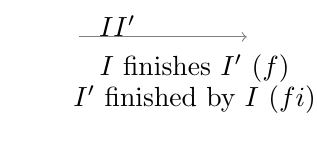
\begin{tikzpicture}[scale=0.5, yscale=0.80]
            \draw[->,gray] (-0.5,0) node[left] {} -- (3.75,0);
            \drawinterval{2.1}{1.7}{3.1}{1.7}{$I$}
            \drawinterval{0}{.7}{3.1}{.7}{$I'$}
            \node[] at (1.5,-1) {$I$ finishes $I'$ ($f$)};
            \node[] at (1.5,-2) {$I'$ finished by $I$ ($fi$)};
        \end{tikzpicture}
        %\caption*{$I$ finishes $I'$ ($f$)\\ $I'$ finished by $I$ ($fi$)}
        \label{subfig:ia:f}
    \end{subfigure}
    \hfill
    \quad
    \hfill
    \caption{Visual representation of all base relations from Allen's Interval Algebra (continuous Intervals)}
    \label{fig:ia}
\end{figure}



 We additionally define the \emph{non-unifiable} relation $\overline{U}$: the relation captures that the union of two intervals is not closed under $\mathbb{I}$. This relation is a special case of the \textit{before} relation: $$\overline{U}([a,b],[c,d]) \text{ iff } ([a,b+1] \text{ before } [c,d]) \sor ([c,d+1] \text{ before } [a,b]) .$$


\begin{example}

We show below examples illustrating some relations between intervals:

\begin{enumerate}
    \item \textbf{Before}: \( I := [0, 3] \) and \( I' := [4, 7] \). \\
    \( I \text{ is before } I' \), since \( I \) ends before \( I' \) starts.

    \item \textbf{Non-unifiable}: \( I := [0,2] \) and \( I' := [4, 7] \). \\
    \( I \text{ is not unifiable with } I' \), since $[0,3]$ precedes $[4,7]$.
    
    \item \textbf{After}: \( I := [5, 8] \) and \( I' := [0, 4] \). \\
    \( I \text{ is after } I' \), since \( I \) starts after \( I' \) ends.
    
    \item \textbf{Meets}: \( I := [0, 3] \) and \( I' := [3, 6] \). \\
    \( I \text{ meets } I' \), since \( I \) ends exactly when \( I' \) starts.
    
    \item \textbf{Overlaps}: \( I := [0, 4] \) and \( I' := [3, 6] \). \\
    \( I \text{ overlaps } I' \), since \( I \) starts before \( I' \) and ends after \( I' \) starts.
    
    \item \textbf{Starts}: \( I := [2, 5] \) and \( I' := [2, 8] \). \\
    \( I \text{ starts } I' \), since \( I \) and \( I' \) have the same start time, but \( I \) ends before \( I' \).
    
    \item \textbf{Finishes}: \( I := [4, 7] \) and \( I' := [1, 7] \). \\
    \( I \text{ finishes } I' \), since \( I \) and \( I' \) have the same end time, but \( I \) starts after \( I' \).
    
    \item \textbf{During}: \( I := [3, 6] \) and \( I' := [1, 8] \). \\
    \( I \text{ is during } I' \), since \( I \) starts after \( I' \) starts and ends before \( I' \) ends.
    
    \item \textbf{Contains}: \( I := [0, 7] \) and \( I' := [2, 5] \). \\
    \( I \text{ contains } I' \), since \( I \) starts before \( I' \) and ends after \( I' \) ends.
    \item \textbf{Non-unifiable}: \( I := [0, 3] \) and \( I' := [5, \infty] \). \\
    \( \overline{U}(I,I') \), since $3+1 < 5$.
\end{enumerate}
\end{example}

\begin{table}[t]
    \centering
    \begin{tabular}{|l|l|l|}
    \hline
        Notation& Interpretation  & Necessary constraints  \\
        \hline
        $\boldsymbol{I< I'}$  & $I$ precedes $I'$  & $\max(I) <_\infty \min(I')$\\
        $\boldsymbol{I' > I}$  & $I'$ precedes $I$  &  \\
        \hline
        $\boldsymbol{I = I'}$  & $I$ is equal to $I'$  & $\min(I) = \min(I')$, $\max(I) = \max(I')$ \\
        & $I'$ is equal to $I$  & \\
        \hline
        $\boldsymbol{I~m~I'}$  & $I$ meets $I'$  & $\max(I) =\min(I')$ \\
        $\boldsymbol{I'~mi~I}$  & $I'$ meets $I$  &  \\
        \hline
        $\boldsymbol{I~o~I'}$  & $I$ overlaps with $I'$  & $\min(I) <_\infty \min(I') < \max(I) <_\infty \max(I')$ \\
        $\boldsymbol{I'~oi~I}$  & $I'$ overlaps with $I$  & \\
        \hline
        $\boldsymbol{I~s~I'}$  & $I$ starts $I'$  & $\min(I) = \min(I')$, $\max(I) <_\infty \max(I')$ \\
        $\boldsymbol{I' si I}$  & $I'$ starts $I$  &  \\
        \hline
        $\boldsymbol{I~d~I'}$  & $I$ during $I'$  & $\min(I') <_\infty \min(I)$, $\max(I) <_\infty \max(I')$ \\
        $\boldsymbol{I'~di~I}$  & $I'$ during $I$  & \\
        \hline
        $\boldsymbol{I~f~I'}$  & $I$ finishes $I'$  & $\max(I) = \max(I')$, $\min(I) >_\infty \min(I')$ \\
        $\boldsymbol{I'~fi~I}$  & $I'$ finishes $I$  &  \\
        \hline
    \end{tabular}
    \caption{Constraint on intervals from $\mathbb{I}$ to satisfy a relation from  Allen's Algebra }
    \label{tab:IAdesc}
\end{table}


The {intersection} operator: $ \cap:\mathbb{I} \times \mathbb{I}  \to \mathbb{I}$  is defined as follows:
	\begin{align*}
		[a,b] \cap [c,d] := 	\left\{
		\begin{array}{lll}
			~	\varnothing & \text{iff} &  [a,b] \text{ before } [c,d]\text{ or } [c,d] \text{ before } [a,b] \\
			~ [max(a, c), min(b,d)] & \text{otherwise}
		\end{array}
		\right.
	\end{align*}

The operators we define now are partially defined as the interval domain not being closed under these operations.

The \emph{union} operator $ \cup:\mathbb{I} \times \mathbb{I}  \rightharpoonup \mathbb{I}$ is partially defined as follows:

 $$[a,b] \cup [c,d] := \begin{cases} 		
		\text{ undefined }& \text{ iff } \overline{U}([a,b],[c,d]) ,\\
		[min(a,b,c,d),max(a,b,c,d)] & \text{otherwise.}
	\end{cases}$$

The partial interval difference operator $\ominus: \mathbb{I} \times \mathbb{I} \rightharpoonup \mathbb{I}$ is the non-commutative, partially defined operation removing all elements from the interval  $I'$ from the interval $I$ in $I \ominus I'$:

$$[a,b] \ominus [c,d] := \begin{cases} 		
		\text{ undefined }& \text{ iff   } [c,d] \text{ during } [a,b],\\
		[a,b] & \text{iff   } [a,b] \cap [c,d]= \emptyset,\\
  \varnothing & \text{iff   } [a,b] \subseteq [c,d],\\
  [a,c-1] & \text{iff   } [a,b] \text{ meets or overlaps or finished by } [c,d],\\
  [d+1,b] & \text{iff   } [c,d] \text{ meets or overlaps or starts by } [a,b].\\
	\end{cases}$$

\begin{example}

Let us consider some examples concerning the operator $\ominus$:

    \begin{itemize}
    \item $
    [2, 8] \ominus [4, 6] = \text{undefined} \quad \text{(during)}$
    
    \item $
    [0, 3] \ominus [5, 7] = [0, 3] \quad \text{(empty intersection)}$
    \item $
    [2, 5] \ominus [1, 6] = \varnothing \quad \text{(subset)}
    $  
    \item $[1, 5] \ominus [3, 7] = [1, 2] \quad \text{(overlaps on left)}$
    \item $[0, 5] \ominus [3, \infty] = [0, 2] \quad \text{(overlaps left with infinity)}$
    \item $[4, 8] \ominus [1, 5] = [6, 8] \quad \text{(overlaps on right)}$
    \item $[3, \infty] \ominus [0, 5] = [6, \infty] \quad \text{(overlaps right with infinity)}$
\end{itemize}


We use now the difference operator on the three-time intervals from our use case:
$I_1 \ominus I_2 = [9,16]\ominus [12,\infty]= [9,11]$. 
On the other hand,
$I_1 \ominus I_3 = [9,16] \ominus [10,14]$ is undefined as $[10,14]$ during $[9,16]$.

\end{example}

\subsection{Interval Sets}
As demonstrated in the previous subsection, the interval domain $\mathbb{I}$ is not closed under union and difference operations. To address this limitation, we introduce the concept of interval sets.
An \emph{interval set}, denoted as $\is$, is a finite set of intervals equipped with a condition to ensure minimal representation.
This condition is called the \emph{canonical form}, which ensures that the interval set contains the smallest number of non-overlapping and non-adjacent intervals necessary to represent a given set of time points.


\begin{definition}[Canonical Interval Set]\label{def:canonis}
An \defn{interval set} $\is$ is said to be in \emph{canonical form} if no two intervals in $\is$ are unifiable. Formally:
\[
\forall \{I, I'\} \subseteq \is: \overline{U}(I, I').
\]
where $\overline{U}(I, I')$ denotes that $I$ and $I'$ are not unifiable (i.e., $I \cup I'$ is not an interval from $\mathbb{I}$).

For the remainder of this paper, we adopt the following notational convention: we use $\is^*$ to refer to interval sets composed exclusively of finite (bounded) intervals. In contrast, we use $\is$ to denote interval sets that may contain infinite intervals, such as those extending to $+\infty$. 

The \emph{size of a set of intervals} $\is$, written $\size{\is}$, is defined as the sum of the sizes of the individual intervals it contains:
\[
\size{\is} := \sum_{I \in \is} \size{I}.
\]
The \emph{cardinality} of the $\is:=\{I_0,I_1, \dots,I_n\}$, written $\card(\is)$, is the number of element intervals in the set,
$\size{\is} := n+1$.
\end{definition}




\begin{example}[Canonical form for interval sets]
Consider the interval set $\is':= \{ [0, 2], [3, 6] \}$. The two intervals forming this interval set are unifiable as $[0, 2] \cup [3, 6] = [0,6]$. The canonical representation is thus $\is := \{ [0, 6] \}$.

Consider the interval set $\is:= \{ [0, 2], [5, 7], [10, \infty] \}$.\\ The pair $[0, 2]$ and $[5, 7]$ satisfy $\overline{U}([0, 2], [5, 7])$.\\ Similarly, $[5, 7]$ and $[10, \infty]$ satisfy $\overline{U}([5, 7], [10, \infty])$.\\ Finally, $[0, 2]$ and $[10, \infty]$ also satisfy $\overline{U}([0, 2], [10, \infty])$.
\end{example}

These representations enable a symbolic encoding of timed constraints, such as those described in our use case. For instance, the obligations from \MA, as shown in Table~\ref{tab:contract}, that an action is permitted \textit{between 02:00 and 04:00, and between 08:00 and 24:00}—can be expressed as the canonical interval set:
\[
\is_3 := \{ [2,4], [8,24] \}.
\]
Similarly, constraints from \DC and \SR can each be represented using singleton interval sets. The constraint \textit{between 09:00 and 16:00}, for example, corresponds to:
\[
\is_1 := \{ [9,16] \},
\]
while \textit{between 10:00 and 14:00} is represented as:
\[
\is_2 := \{ [10,14] \}.
\]
We adopt this interval-set representation as a uniform basis for the symbolic manipulation of temporal constraints within the logical framework developed in the following sections.

\begin{definition}[Expansion Factor of an Interval Set]
\label{def:expansion-factor}
Let \(\is\) be a finite set of intervals. The \defn{expansion factor} \(\expf(\is)\) of \(\is\) is defined as the ratio between the total number of discrete points covered by the intervals in \(\is\) and the number of intervals in \(\is\), i.e.,
\[
\expf(\is) := \frac{\size{\is}}{\card(\is)}\quad,
\]
where \(\size{\is}\) is the sum of the sizes (number of points) of the intervals in \(\is\), and \(\card(\is)\) is the number of intervals in \(\is\).
\end{definition}

\begin{example}[Minimal Expansion Factor]
Consider the interval set
\[
\is_1 = \{ [3,3], [5,5], [10,10] \}.
\]
The cardinality is $\card(\is_1) = 3$, and the size is
\[
\size{\is_1} = (3 - 3 + 1) + (5 - 5 + 1) + (10 - 10 + 1) = 1 + 1 + 1 = 3.
\]
Therefore, the expansion factor is
\[
\expf(\is_1) = \frac{3}{3} = 1,
\]

\end{example}

\begin{example}[Large Expansion Factor]
Consider now the interval set
\[
\is_2 = \{ [1,1000], [1050,1050], [2000,2000] \},
\]
which consists of one large interval and two punctual intervals. Here,
\[
\card(\is_2) = 3,
\]
and
\[
\size{\is_2} = (1000 - 1 + 1) + (1050 - 1050 + 1) + (2000 - 2000 + 1) = 1000 + 1 + 1 = 1002.
\]
Thus, the expansion factor is
\[
\expf(\is_2) = \frac{1002}{3} = 334,
\]
Showing a large blow-up, mainly caused by the large intervals.
\end{example}

\subsection{Arithmetic of Interval Sets}\label{isarithmetic}
    \paragraph{Sub-element} An interval $I$ is a \emph{sub-element} of $\mathfrak{I}$ (written $I \subin \mathfrak{I}$) if it is included in one of the elements of the set of intervals. We write:
    $ I \subin \mathfrak{I} \text{ iff } \exists I' \in \mathfrak{I} : I \subseteq I' $. We abuse the notation for time points $t  \in \mathbb{N}$ and write $t \subin \mathfrak{I}$ iff $[t,t] \subin \mathfrak{I}$.

    \paragraph{Inclusion} We say $\mathfrak{I}$ is \emph{included} in $\mathfrak{I}'$ and write:
     $\mathfrak{I} \subset \mathfrak{I}' \text{ iff } \forall I \in \mathfrak{I} ~\exists I' \in \mathfrak{I}': I \subset I'$.

    \begin{example} Given $\mathfrak{I}:= \{ [1, 4], [6, 9] \}$:
    \begin{itemize}
        \item The interval $[2, 3] \subin \mathfrak{I}$ because $[2, 3] \subseteq [1, 4] \in \mathfrak{I}$.
        \item The time point $7 \subin \mathfrak{I}$ because $[7, 7] \subseteq [6, 9] \in \mathfrak{I}$.
    \end{itemize}
%    \end{example}

    Let $\mathfrak{I'} = \{ [0, 4], [6, \infty] \}$. Then $\mathfrak{I} \subseteq \mathfrak{I'}$ since
    \begin{itemize}
        \item $[1, 4] \subseteq [0, 4] \in \mathfrak{I'}$,
        \item $[6, 9] \subseteq [6, \infty] \in \mathfrak{I'}$.
    \end{itemize}
    
    For the sets of intervals $\is_1:= \{[9,16]\}$ and $\is_3:=\{[2,4],[8,24]\}$ from 
    our use case we have: $\is_1 \subset \is_3$.
    \end{example}

    \paragraph{Intersection} The intersection of two sets of intervals $\mathfrak{I}$ and $\mathfrak{I}'$ is the set of intervals containing all the intervals present in both interval sets. The operator is commutative and is defined as:
    $$
    \mathfrak{I} \cap \mathfrak{I}' :=\begin{cases}
     \emptyset& \text{if } \forall I\in \mathfrak{I}, \forall I'\in \mathfrak{I}': I \cap I'=\varnothing,\\
     \{ I \cap I' \mid I \in \mathfrak{I}, I' \in \mathfrak{I}', I \cap I' \neq \varnothing \} & \text{otherwise}.
    \end{cases}
    $$

    \begin{example} Consider the following examples:
    \begin{itemize}
        \item If $\mathfrak{I}:= \{ [1, 5], [8, 10], [19,\infty] \}$ and $\mathfrak{I}':= \{ [3, 7], [9, 12] \}$, we have $\mathfrak{I}\cap \mathfrak{I}' = \{ [3, 5], [9, 10] \}$,\\ as $[1, 5] \cap [3, 7] = [3, 5]$ and $[8, 10] \cap [9, 12] = [9, 10]$.
        \item If $\mathfrak{I} := \{ [1, 5], [8, 10] \}$ and $\mathfrak{I}':= \{ [6, 7], [12, \infty] \}$ then $\mathfrak{I}\cap \mathfrak{I}' = \emptyset$ (as none of the intervals from $\mathfrak{I}$ intersect with any interval from $\mathfrak{I}'$).
    \end{itemize}

    For the intervals $\is_1$, $\is_2$, and $\is_3$ related respectively to $\DC$, $\SR$, and $\MA$ from 
    the use case:
    \begin{itemize}
        \item $\is_1 \cap \is_2= \{[9,16]\} \cap \{[10,14]\}= \{[10,14]\}$.
        \item $\is_1 \cap \is_3 = \{[9,16]\} \cap \{[2,4],[8, 24]\}= \{[9,16]\}$.
    \end{itemize}
\end{example}


 \subsubsection{Union}
The union of two interval sets $\is$ and $\is'$ is recursively computed by the successive union of each interval $I_i \in \is'$ with $\is$:

\[
\is \cup \is' := \left\{ \left( \left(\is \cup I_1) \cdots \right) \cup I_n \right) \ \middle|\ I_1, \dots, I_n \in \is' \right\}.
\]


The union of an interval set $\is$ with a single interval $I$ is given by:
\[
\is \cup I := \left\{ \left( \bigcup_{I_i \in U(I, \is)} (I \cup I_i) \right) \right\} \circ \overline{U}(I, \is),
\]

where $\circ$ denotes set concatenation, and the subset of unifiable and non unifiable interval with $I$ from $\is$ are defined as:
\begin{align*}
\overline{U}(I, \is) &:= \{ I_i \in \is \mid \overline{U}(I, I_i) \}, \\
U(I, \is) &:= \{ I_i \in \is \mid I_i \notin \overline{U}(I, \is) \}.
\end{align*}

\begin{example} Let \(\is := \{ [1, 5], [9, 11] \}\) and \(\is' := \{ [3, 7], [9, 12] \}\):
\begin{align*}
\is \cup \is' &= \big(\{ [1, 5], [9, 11] \}\cup [1,7]\big) \cup [9,12] &\text(unrolling)\\
&= \big( \{ [1,5] \cup [3,7]\} \circ\{ [9,11]\}\big) \cup [9,12]  & (\text{as~}  \overline{U}([9,11], [3,7]))\\
&=\{[1,7],[9,11]\} \cup [9,12] & \text{(simplification)}\\
&= \{ [9,11] \cup [9,12] \} \circ \{[1,7]\}  & (\text{as~}\overline{U}([9,12], [1,7]))\\
&= \{[1,7],[9,12]\}
\end{align*}
\end{example}

\subsubsection{Difference (Reduction)}\label{differenceop}

The \emph{difference} of an interval set $\is$ by an interval set $\is'$, denoted $\is \ominus \is'$, is the set of intervals in $\is$ excluding those that overlap with $\is'$:

$$\is \ominus \is' := \bigcup_{I_i \in \is}(I \ominus \is') \text{ with } I \ominus \mathfrak{I'}= \bigcap_{I_i \in \is'}(I \ominus I_i).$$
Where the \emph{redefined} reduction of two intervals is now computed as \emph{set of intervals} instead of intervals as defined in the arithmetic of intervals: $\ominus: \mathbb{I} \times \mathbb{I} \to 2^\mathbb{I}$ is defined as :
	$$[a,b] \ominus [c,d] := \begin{cases} 		
		\{[a,c-1], [d+1,b]\}& \text{ iff   } [c,d] \text{ during } [a,b],\\
		\{[a,b]\} & \text{iff   } [a,b] \cap [c,d]= \varnothing,\\
  \emptyset & \text{iff   } [a,b] \subseteq [c,d],\\
  \{[a,c-1]\} & \text{iff   } [a,b] \text{ meets or overlaps or finished by} [c,d],\\
  \{[d+1,b]\} & \text{iff   } [c,d] \text{ meets or overlaps or starts by} [a,b].\\
	\end{cases}$$
    
\begin{remark}
An alternative definition could be $I \ominus I' := \{I_i \mid I_i \subseteq I \text{ and } I_i \not\subseteq I'\}.$ 
\end{remark}

\begin{example} Let $\is = \{ [1, 10] \}$ and $\is' = \{ [3, 5],\ [7, 8] \}$:

\begin{itemize}
    \item $[1, 10] \ominus [3, 5]= \{[1,2], [6,10]\}$.
    \item $[1, 10] \ominus [7, 8]= \{[1,6], [9,10]\}$.
\end{itemize}
\end{example}

Thus, $\is \ominus \is' = \{ [1, 2],\ [6, 6],\ [9, 10] \}$.

From the intervals $\is_1, \is_2, \is_3$ related to our three normative systems from the use case, we have:
\begin{itemize}
    \item $\is_1 \ominus \is_2= \{[9,16]\} \ominus \{[10,14]\}= \{[9,9],[15,16]\}.$
    \item $\is_1 \ominus \is_3 = \{[9,16]\} \ominus \{[2,4],[8, 24]\}= \emptyset. $
\end{itemize}

\section{Discrete-Action Word Models}\label{traces}
Since our normative specifications constrain what agents ought to do, we take discrete actions as primitive and represent executions as discrete-action words.
In contrast to control-theoretic and physical models based on continuous signals or state trajectories, our setting is action-centric: we record which actions occur, and we reason about their order and, when needed, their timing.
Accordingly, a word is a sequence of discrete events that captures ``what happened'', rather than a valuation that describes ``what holds'' over time.
These words form the basic semantic objects for the logics developed in subsequent chapters.
When we speak of traces, we mean recorded words obtained from concrete executions.

We begin by establishing three word models of action-based behavior and the canonical morphisms between them. Subsequently, we study how to synchronize two words of the same type.

\subsection{An Abstract Algebraic Theory of Discrete-Action Words}
For the remainder of this dissertation, let \(\Sigma\) denote a non-empty set of discrete \emph{actions}. Before introducing the three timing models, we fix a small algebraic core that is shared by all discrete-action words, namely the basic sequence structure and the standard operators that act on it.

Words are sequences of events. An \emph{event} in our discrete setting, denoted by $\event$, is a data structure derived from $\Sigma$. We denote the set of \emph{finite words} by $\event^\star$, the set of \emph{infinite words} by $\event^\omega$, and the set of all words (finite or infinite) by $\event^\infty := \event^\star \cup \event^\omega$.
Before moving to the differences regarding timing models, all word types share the fundamental algebraic structure of a sequence. To avoid redundancy in subsequent definitions, we establish here the properties common to any finite word $w$ over a concrete event domain $E$ (where $E$ could simply be $\Sigma$).

\paragraph{Notation for finite traces} \( w = \trace{e_1,\,e_2,\,\dots,\,e_{n}} \in \mathbb{E}^* \) symbolizes a finite word $w$ defined by a sequence of events $e_i$ from \( E \). We define the following canonical notions:

\paragraph{Notation for finite traces.}
Let \( w = \trace{e_1,\,e_2,\,\dots,\,e_{n}} \in E^* \) be a finite word.
We adopt \emph{1-based indexing} where indices correspond to the count of events.

\begin{itemize}
    \item \defn{Size}: The length of the word is denoted by \( |w| := n \).
    
    \item \defn{Positions}: The set of valid element indices is \( \mathsf{pos}(w) := \{1, 2, \dots, n\} \).
    
    \item \defn{Indexing}: For any \( k \in \mathsf{pos}(w) \), the event at position \(k\) is \( w[k] := e_k \).
    
    \item \defn{Prefix}: For any \( 0 \le k \le n \), the prefix of length \( k \) is denoted by \( w_k \) (or \( w[1,k] \)).
    \[
        w_k := \trace{e_1, \dots, e_k}.
    \]
    \emph{Exception Handling:} If \( k=0 \), then \( w_0 = \emptytrace \).
    
    \item \defn{Suffix}: For any \( 0 \le k \le n \), the suffix remaining \emph{after} the first \( k \) events is denoted by \( w^k \).
    \[
        w^k := \trace{e_{k+1}, \dots, e_n}.
    \]
    \emph{Exception Handling:} If \( k=n \), then \( w^n = \emptytrace \).
    
    % \item \defn{Decomposition}: For any cut point \( 0 \le k \le n \), the word is the concatenation of prefix and suffix:
    % \[
    %     w = w_k \concat w^k.
    % \]
\end{itemize}
\paragraph{Words vs. traces.}
Although we conceptually distinguish a \emph{word} as an abstract behavior from a \emph{trace} as an observed execution, finite words and finite traces boil down to the same underlying data structure, namely a finite sequence of events. Accordingly, in the scope of this dissertation, we use \emph{word} as the default technical term in the formal development, and we use \emph{trace} only when emphasizing that a particular finite sequence comes from recorded observations.

\paragraph{Omega notation for infinite words.}
Let $\event$ be the underlying event domain.
For any nonempty finite word $u \in \event^{+}$, written $u=\trace{e_1,\dots,e_n}$ with $n\ge 1$, we write
$u^{\omega}$
to denote the infinite word obtained by repeating $u$ indefinitely, that is,
\[
u^{\omega} \;:=\; \trace{e_1,\dots,e_n,\,e_1,\dots,e_n,\,e_1,\dots,e_n,\,\dots} \;\in\; \event^{\omega}.
\]


\noindent\textbf{Generic Projection.}
For a subset of events $S \subseteq E$, the projection $w{\upharpoonright}S$ is the subsequence obtained by deleting all events $e_k$ such that $e_k \notin S$.


\subsection{Logical-Time Words}

Logical-time words capture \emph{order only}, abstracting away any notion of specific timing. They are the staple semantic objects in interleaving models of process calculi (such as CCS\cite{Milner89} and CSP\cite{hoare1978communicating}). Moreover, in Mazurkiewicz trace theory, one starts from strings over an alphabet and then forms \emph{traces} by identifying strings that differ only by swapping adjacent independent actions (that is, a trace is an equivalence class of words modulo an independence relation) \cite{diekert1995book}.

\begin{definition}[Logical-time word, notation \(\tault\)]
  A (finite) logical-time word over an alphabet \(\Sigma\) is a sequence:
  \[
  \tault\;=\; \trace{(a_1),\,(a_2),\,\dots,\,(a_{n})}\ \in\ \Sigma^{*},
  \]
  where \(a_k\in\Sigma\) for all \(k\in\{1,\dots,n\}\).
\end{definition}

We now introduce basic operators on logical-time words. We start with concatenation, then define a counting function for action occurrences. Both notions will be reused when relating logical-time words to the richer time models introduced next.


%
\begin{definition}[Concatenation of logical-time words]
  Let $\tault_1=\trace{(a_1),\dots,(a_{n})}\in\Sigma^{*}$ and
  $\tault_2=\trace{(b_1),\dots,(b_{m})}\in\Sigma^{*}$.
  Their \defn{concatenation}, written $\tault_1\concat\tault_2$, is the logical-time word in $\Sigma^{*}$ defined by
  \[
    \tault_1 \concat \tault_2
    \;:=\;
    \trace{(a_1),\dots,(a_{n}),(b_1),\dots,(b_{m})}.
  \]
  \[
    \tault_1 \concat \emptytrace
    \;:=\;
    \tault_1.
  \]
  \[
    \emptytrace \concat \tault_2
    \;:=\;
    \tault_2.
  \]
\end{definition}


Additionally, the following holds for the concatenation of any two logical-time words:
\begin{itemize}
  \item \defn{Length}: $\lvert\tault_1\concat\tault_2\rvert = \lvert\tault_1\rvert + \lvert\tault_2\rvert$.
  \item \defn{Indexing}: for $k\in\mathsf{pos}(\tault_1\concat\tault_2)$,
  \[
  (\tault_1\concat\tault_2)[k] :=
  \begin{cases}
    \tault_1[k], & \text{if } 1\le k \le \lvert\tault_1\rvert,\\
    \tault_2[k-\lvert\tault_1\rvert], & \text{if } \lvert\tault_1\rvert < k \le \lvert\tault_1\rvert+\lvert\tault_2\rvert.
  \end{cases}
  \]
\end{itemize}

The next operator abstracts from positions and records how often a given action occurs in a word.

\begin{definition}[Counting function on logical-time words]
  Let $a\in\Sigma$ and let $\tault=\trace{(a_1),\dots,(a_{n})}\in\Sigma^{*}$ be a logical-time word.
  The \defn{count} of $a$ in $\tault$, written $\#(a,\tault)$, is defined by
  \[
    \#(a,\tault)
    \;:=\;
    \big|\{\, k\in\mathsf{pos}(\tault) \mid \tault[k]=a \,\}\big|.
  \]
\end{definition}



\begin{example}[Logical-time operators]
  Let \( \Sigma=\{\textsf{pick},\textsf{handover}\} \).
  Consider the word:
  \[
  \tault=\trace{(\textsf{pick}),(\textsf{handover})}.
  \]
  \emph{Size and Indexing:} \(|\tault|=2\), \(\tault[1]=\textsf{pick}\).\\
  \emph{Counts:} \(\#({\textsf{handover}},\tault)=1\).\\
  \emph{Projection:} with \(A=\{\textsf{handover}\}\), \(\tault{\upharpoonright}A=\trace{(\textsf{handover})}\).\\
  \emph{Concatenation:} \(\tault\concat\trace{(\textsf{pick})} = \trace{(\textsf{pick}),(\textsf{handover}),(\textsf{pick})}\).
\end{example}


\subsection{Metric-Timed Words}
\noindent\textbf{Context.}
Metric-timed words extend the previous model by recording \emph{which} action occurs and \emph{when} it occurs. They are defined in research works on timed automata \cite{DBLP:journals/tcs/AlurD94}.

\begin{definition}[Finite \timedwords of actions] \label{timedwords} 
    A \emph{finite \timedword} $\tau$ is defined as a finite sequence of timed events, $\tau \in ({\timedevents})^*$.
     \[\tau := \trace{(a_1,t_1), (a_2,t_2), \ \dots, \ (a_{n},t_{n}) }\]
     with \(a_k\in\Sigma\), \(t_k\in\mathbb{N}\), and strictly increasing timestamps \(0\le t_1<\cdots<t_{n}\).
\end{definition}

% NOTE: The definition name is left as is, but the surrounding prose and references should use "words"
\begin{definition}[Auxiliary operators on metric-timed words]
  Let $\taumt=\trace{(a_1,t_1),\dots,(a_{n},t_{n})}\in(\Sigma\times\mathbb{N})^{*}$.
  \begin{itemize}
    \item The \defn{label} and \defn{timestamp} projections of the $k$th event are defined by
    \[
      \mathsf{lab}(\taumt,k):=a_k,\qquad \mathsf{ts}(\taumt,k):=t_k\qquad (k\in\mathsf{pos}(\taumt)).
    \]
    \item The \defn{time set} of $\taumt$ is
    \[
      \mathsf{time}(\taumt):=\{\, t_k \mid k\in\mathsf{pos}(\taumt)\,\}.
    \]
    \item The \defn{last time point} is defined by
    \[
      \mathsf{last}(\taumt):=
      \begin{cases}
        t_n, & \text{if } n>0,\\
        0, & \text{if } n=0.
      \end{cases}
    \]
    \item The \defn{time span} is
    \[
      \mathsf{span}(\taumt):=
      \begin{cases}
        t_n-t_1, & \text{if } n>0,\\
        0, & \text{if } n=0.
      \end{cases}
    \]
    \item For $a\in\Sigma$, the \defn{count} of $a$ in $\taumt$ is
    \[
      \#(a,\taumt):=\big|\{\, k\in\mathsf{pos}(\taumt) \mid \mathsf{lab}(\taumt,k)=a \,\}\big|.
    \]
  \end{itemize}
\end{definition}

    We refer by $\domtr$ to the domain of finite \timedwords. Unlike the logical-time setting, where one can only compare events by their order, metric-timed words support quantitative reasoning about timing. In particular, the operators on logical-time words, such as concatenation and counting, do not determine any numerical distance between events. The next two definitions exploit the additional timestamp component: $\Delta$ measures the elapsed time between two positions, while $\rho$ looks up which action, if any, occurs at a given absolute time point.


    \begin{definition}[Timed distance between two events]
        Let $\taumt=\trace{(a_1,t_1),\dots,(a_{n},t_{n})}\in(\Sigma\times\mathbb{N})^{*}$ be a metric-timed word.
        For any two indices $i,j\in\mathsf{pos}(\taumt)$ with $i<j$, the \defn{timed distance} between event $i$ and event $j$ is
        \[
          \Delta(\taumt,(i,j))\;:=\; t_j-t_i.
        \]
      \end{definition}
    
     \begin{definition}[Action Lookup Function]\label{defrho}
     
     The \emph{action lookup function} $\rho : \domtr \times \mathbb{N} \to \Sigma \cup \{ \Undef \}$ returns the action performed at absolute time $t$ in a metric-timed word; if no event occurs at time $t$, it returns the special symbol $\Undef$:
        \[
        \rho\big(\trace{(a_1,t_1), \dots, (a_{n},t_{n})}, t\big) := 
        \begin{cases} 		
            a_i & \text{if  } t_i=t \text{ for some } i \in \{1,\dots,n\},\\
            \Undef & \text{otherwise.}
        \end{cases}
        \]
    \end{definition}


\noindent\textbf{Basic operators and short hands.}
For \(A\subseteq\Sigma\), projection \( \taumt{\upharpoonright}A\in(A\times\mathbb{N})^{*} \) keeps exactly the pairs \((a,t)\) where \(a\in A\).\\
Prefixes can be defined by \emph{length} \( \taumt[1,k] \), or by \emph{time} \( \taumt{\upharpoonright}\{t\le T\} \) (shorthand: \( \taumt\{t\le T\}\)).\\


\begin{example}[Metric-timed operators]
  Consider an alphabet $\Sigma=\{\textsf{badge\_tapped},\textsf{door\_open}\}$.
  \[
  \taumt=\trace{(\textsf{badge\_tapped},1),(\textsf{door\_open},3)}.
  \]
  \emph{Size and Indexing:} \(|\taumt|=2\), \(\taumt[1]=(\textsf{badge\_tapped},1)\).\\
  \emph{Lookup action:} $\rho(\taumt,1)=\textsf{badge\_tapped}$ and $\rho(\taumt,2)= \Undef$.\\
  \emph{Time properties:} \(\mathsf{time}(\taumt)=\{1,3\}\), \(\mathsf{span}(\taumt)=2\).\\
  \emph{Time-prefix:} \(\taumt\{t\le 2\}=\trace{(\textsf{badge\_tapped},1)}\).\\
  \emph{Timed distance}: the distance between event $1$ and event $2$ is $\Delta(\taumt,(1,2))=3-1=2$.
\end{example}

Metric-timed words provide \emph{precise} quantitative information, in particular the exact timed distance between any two events in the same word, captured by differences of their timestamps.
For this model, concatenation is not defined for arbitrary pairs of words: if two words both contain an event at the same time point, then concatenating them would violate the requirement of strictly increasing timestamps. Hence, concatenation is only defined when the timestamp sets are disjoint and the last time point of the first word is strictly smaller than the first time point of the second word.


\subsection{Synchronous-Time Words}
Synchronous-time words represent behavior under a single global logical clock. Each tick corresponds to one round of computation, and inactivity is made explicit via the stutter symbol ``$-$''. This model underlies synchronous languages such as Esterel\cite{berry1984esterel}, Lustre\cite{Halbwachs93}, and LoLa\cite{d2005lola}.

\paragraph{The synchronous hypothesis.}
The synchronous hypothesis fixes the intended abstraction level: within one clock cycle, the system reads its inputs, computes the next state, and emits its outputs within the same logical instant. Computation is therefore treated as taking zero time, and time advances only between cycles. Accordingly, behavior is naturally represented as a word indexed by $\mathbb{N}$, where each position corresponds to one tick and records the global observation at that tick, for instance as a global state or as a set of events. Related synchronous process-algebra variants also exist, most notably Milner's synchronous CCS (SCCS), which adopts the same global-clock view and interprets behavior as lockstep rounds of actions \cite{milner1983calculi}.

\begin{definition}[Synchronous-time word, notation \(\taust\)]
  Fix an alphabet \(\Sigma\) and a stutter symbol ``\(-\)'' with \( -\notin\Sigma \).
  A (finite) \emph{synchronous-time word} is a finite sequence of events over $(\Sigma\cup\{-\})$
  \[
  \taust \;=\; \trace{(s_0),\,(s_1),\,\dots,\,(s_T)} \ \in\ (\Sigma\cup\{-\})^{*},
  \]
  where \(s_t\in\Sigma\cup\{-\}\) represents the observation at round \(t\) and \(T\) is called the \defn{horizon}.
\end{definition}

Synchronous-time words sit between logical-time words and metric-timed words. Like logical time, they are discrete sequences, but they come with an explicit global round index that plays the role of a coarse clock. Like metric time, one can talk about \emph{when} something happens, but only in terms of round numbers rather than absolute timestamps. The crucial difference to both earlier models is that the \emph{absence} of an action is itself observable, represented by the stutter symbol ``$-$''.


  

\noindent\textbf{Basic operators and short hands.}
For \(A\subseteq\Sigma\):
\begin{itemize}
  \item \defn{Stutter-preserving projection} \( \taust{\upharpoonright}A \in (A\cup\{-\})^{*} \) keeps letters in \(A\) and all ``\(-\)''.
  \item \defn{Logical (stutter-erasing) projection} \( \erase_{-}(\taust{\upharpoonright}A)\in A^{*} \) drops all ``\(-\)''.
\end{itemize}
For $a\in\Sigma$, the \defn{count} of $a$ in $\taust$ is $\#(a,\taust):=\big|\{\, t\in\mathsf{pos}(\taust)\mid \taust[t]=a \,\}\big|$, and the set of \defn{active rounds} is $\mathsf{act}(\taust):=\{\, t\in\mathsf{pos}(\taust)\mid \taust[t]\neq - \,\}$.
The round-prefix is denoted \( \taust[0,r]:=\trace{(s_0),\dots,(s_r)} \) for \(0\le r\le T\).

\begin{example}[controller at 1\,Hz, illustrating all operators]
    Consider HVAC (Heating, Ventilation, and Air Conditioning) actuator (1) and a security Sensor (2), both controlled by a synchronous controller:
    \[
    \Sigma_1=\{\textsf{heat\_on}\},\qquad 
    \Sigma_2=\{\textsf{door\_lock}\}.
    \]
    In one episode, we record
    \[
    \taust_1=\trace{(-),(-),(\textsf{heat\_on})},\qquad
    \taust_2=\trace{(-),(\textsf{door\_lock}),(-)}.
    \]
    
    \noindent\emph{Size, positions, indexing:}\\
    \(|\taust_1|=|\taust_2|=3\) with horizon \(T=2\),  
    \(\mathsf{pos}(\taust_1)=\{0,1,2\}\),  
    \(\taust_1[2]=\textsf{heat\_on}\).
    
    \noindent\emph{Counts and active rounds:}\\
    \(\#(\textsf{heat\_on},\taust_1)=1\),  
    \(\mathsf{act}(\taust_1)=\{2\}\).
    
    \noindent\emph{Stutter-preserving projection:}\\
    with \(A=\emptyset\),  
    \(\taust_1{\upharpoonright}A=\trace{(-),(-),(-)}\).
    
    \noindent\emph{Logical (stutter-erasing) projection:}\\
    \(\erase_{-}(\taust_1{\upharpoonright}A)=\emptytrace\),  
    while \(\erase_{-}(\taust_1)=\trace{(\textsf{heat\_on})}\).
    
    \noindent\emph{Round-prefix:}\\
    \(\taust_2[0,1]=\trace{(-),(\textsf{door\_lock})}\).
    
    \end{example}
  

% --- Summary diagram and explanation inserted here ---
\subsection{Connecting the Three Action Word Models}
The objective of this subsection is to connect the three action-centric word models introduced above. Given a metric-timed word \(\taumt\), we introduce two canonical morphisms that deliberately discard part of the information: the \emph{logical-time projection} \(\LT\), which erases time stamps while preserving the order of events, and the \emph{synchronous padding} \(\ST\), which aligns events to a global round clock by inserting explicit stutter symbols ``\(-\)''. We set up the clock frequency of the synchronous-time word to correspond to a single unit of metric time.

\noindent\textbf{Summary diagram.}
Figure~\ref{fig:word-models-summary} summarizes the relationship between the three word models using a running toy example with two events. Starting from a metric-timed word, synchronous padding $\ST$ aligns events to a global round clock by inserting explicit stutters ``$-$'', and logical projection $\LT$ forgets timing information and retains only the event order. The diagram also makes explicit that the codomain changes across the mappings: $\ST$ moves from timed event pairs to round-indexed letters, whereas $\LT$ yields a pure order-only word.

\begin{figure}[t]
\centering
\begin{tikzpicture}[
    node distance=1.5cm,
    font=\sffamily,
    event/.style={circle, draw=blue!80, fill=blue!10, thick, minimum size=8mm, inner sep=0pt},
    stutter/.style={circle, draw=gray!50, fill=gray!10, dashed, minimum size=6mm, inner sep=0pt},
    label text/.style={font=\bfseries\small, align=left},
    axis/.style={->, >=Latex, thick, gray},
    map line/.style={->, dashed, color=gray!80, shorten >=2pt, shorten <=2pt}
]

    % --- 1. Metric-Timed Word (Top Layer) ---
    \node[label text] (mt_label) at (-2, 0) {Metric-Timed\\ $\tau_{mt}$};

    \draw[axis] (0,0) -- (8,0) node[right] {time ($t$)};

    \node[event, label=above:{$t=1$}] (m1) at (2, 0) {$a$};
    \node[event, label=above:{$t=3$}] (m2) at (6, 0) {$b$};

    \foreach \x in {0,1,2,3,4} \draw[gray] (\x*2, 0.1) -- (\x*2, -0.1);
    \node[below, gray, font=\tiny] at (0,0) {0};
    \node[below, gray, font=\tiny] at (4,0) {2};
    \node[below, gray, font=\tiny] at (8,0) {4};

    % --- 2. Synchronous-Time Word (Middle Layer) ---
    \node[label text] (st_label) at (-2, -2.5) {Synchronous\\ $\tau_{st} = \ST(\tau_{mt})$};

    \draw[axis] (0,-2.5) -- (8,-2.5) node[right] {rounds};

    \node[stutter, label=below:{\scriptsize 0}] (s0) at (0, -2.5) {$-$};
    \node[event, label=below:{\scriptsize 1}]  (s1) at (2, -2.5) {$a$};
    \node[stutter, label=below:{\scriptsize 2}] (s2) at (4, -2.5) {$-$};
    \node[event, label=below:{\scriptsize 3}]  (s3) at (6, -2.5) {$b$};

    \draw[map line] (m1) -- (s1);
    \draw[map line] (m2) -- (s3);

    % --- 3. Logical-Time Word (Bottom Layer) ---
    \node[label text] (lt_label) at (-2, -5) {Logical-Time\\ $\tau_{lt} = \LT(\tau_{mt})$};

    \node[event] (l1) at (3, -5) {$a$};
    \node[event] (l2) at (5, -5) {$b$};

    \draw[->, thick, shorten >=1pt] (l1) -- (l2);

    \draw[map line] (s1) -- (l1);
    \draw[map line] (s3) -- (l2);

    \node[right, gray, font=\footnotesize, align=left] at (8.5, -1.25)
        {\textbf{Synchronous Padding} $\ST$\\
         Aligns events to clock ticks\\
         Inserts `$-$' where needed};

    \node[right, gray, font=\footnotesize, align=left] at (8.5, -3.75)
        {\textbf{Logical Projection} $\LT$\\
         Forgets time and stutters\\
         Preserves order only};

\end{tikzpicture}
\caption{Relationship between metric-timed, synchronous-time, and logical-time word models, and the forgetful morphisms $\ST$ and $\LT$ on a running example.}
\label{fig:word-models-summary}
\end{figure}

% The following paragraphs now refer to "word models" and "words"
\paragraph{From metric time to logical time.}
The map \(\LT\) drops time stamps but preserves labels and their order. It is the coarsest view that still distinguishes different event sequences.

\begin{lemma}[Logical-time projection \(\LT\): order-only view]
Let \(\taumt=\trace{(a_1,t_1),\dots,(a_{n},t_{n})} \) be a timed word. There exists a unique logical word \(\tault=\LT(\taumt)\in\Sigma^{*}\) satisfying:
\begin{itemize}
  \item \textbf{Number of event preservation}: \( |\tault| = |\taumt| = n \).
  \item \textbf{Action occurrence preservation}: \( \forall a\in\Sigma, \#(a,\tault) = \#(a,\taumt) \).
  \item \textbf{Event order preservation}: If \(\taumt[k]\) precedes \(\taumt[\ell]\), then \(\tault[k]\) precedes \(\tault[\ell]\) in \(\tault\).
  \item \textbf{Projection compatibility}: \( \forall A\subseteq\Sigma, (\LT(\taumt)){\upharpoonright}A = \LT(\taumt{\upharpoonright}A) \).
  \item \textbf{Timing is forgotten}: \(\LT\) is invariant under strictly increasing retiming of timestamps.
\end{itemize}
\end{lemma}

\begin{proof}
\defn{Construction.}\;
Define \(\LT(\taumt):=\trace{(a_1),\,(a_2),\,\dots,\,(a_{n})}\). All properties follow from erasing time stamps while preserving labels and their order.
\end{proof}

\paragraph{From metric time to synchronous time.}
The map \(\ST\) aligns events to a global round clock by inserting ``\(-\)'' at rounds with no event; erasing ``\(-\)'' brings us back to logical time.

\begin{lemma}[Synchronous padding \(\ST\): round-indexed view]
Let \(\taumt\) be a metric-timed word, and assume one synchronous tick per metric unit. There exists a unique synchronous word \(\taust=\ST(\taumt)\in(\Sigma\cup\{-\})^{*}\) such that, writing \(T:=\mathsf{last}(\taumt)\) when \(|\taumt|>0\):
\begin{itemize}
  \item \textbf{Size / horizon relation}: If \(|\taumt|>0\), \(|\ST(\taumt)| = T+1\) and \(\mathsf{pos}(\ST(\taumt))=\{0,\dots,T\}\).
  \item \textbf{Exact time-of-occurrence}: For any \(t\), \(\ST(\taumt)[t] = \mathsf{lab}(\taumt,k)\) if \(t=\mathsf{ts}(\taumt,k)\), otherwise it is \(-\).
  \item \textbf{Active rounds}: \(\mathsf{act}(\ST(\taumt)) = \mathsf{time}(\taumt)\).
  \item \textbf{Preservation of occurrences}: \(\forall a\in\Sigma, \#(a,\ST(\taumt)) = \#(a,\taumt)\).
  \item \textbf{Equivalence to logical time}: \(\erase_{-}(\ST(\taumt)) = \LT(\taumt)\).
\end{itemize}
\end{lemma}

\begin{proof}
\defn{Construction.}\;
If \(|\taumt|=0\), set \(\ST(\taumt):=\emptytrace\). Otherwise let \(T:=\mathsf{last}(\taumt)\). For every \(t\in\{0,\dots,T\}\), define \(\ST(\taumt)[t]\) to be \(a_k\) if \(t=t_k\) for some \(k\), and \(-\) otherwise. Each property follows directly from this definition and the strict monotonicity of timestamps.
\end{proof}

\paragraph{On non-invertibility.}
Both \(\LT\) and \(\ST\) are \emph{many-to-one}. In particular, \(\LT\) is \emph{not} invertible. One cannot reconstruct a unique metric or synchronous word from logical time alone. Conversely, given \(\ST(\taumt)\) under the one-tick-per-unit assumption, the timestamps are recoverable from the indices of non-stutter symbols, up to the chosen time unit and the choice of time origin.

\paragraph{Takeaway.}
\(\LT\) and \(\ST\) are the canonical forgetful maps from metric time to, respectively, order-only and round-synchronous views. They preserve exactly the event properties listed above and discard the rest.

\subsection{Synchronization of Words}\label{operators}

\noindent\textbf{Design rationale.}
Having defined words for generic systems, we now turn to the interaction between systems. Different communities fix different \emph{time assumptions}, which determine how local words are aligned. Process calculi (CCS/CSP) adopt \emph{no global clock} and reason over order only, yielding \emph{pure interleaving} and optionally \emph{shared action handshakes}. Synchronous languages assume a \emph{single global round clock} (lockstep). Timed automata use \emph{absolute timestamps} and synchronize at equal times on shared actions.

In this section, we instantiate three operators consistent with our models for two specific agents, denoted by indices 1 and 2, with alphabets $\Sigma_1$ and $\Sigma_2$. We cover:
(i) \emph{asynchrony} on logical-time words (\(\tault\)),
(ii) \emph{lockstep synchrony} on synchronous words (\(\taust\)),
and (iii) \emph{synchronous handshake} on synchronous words with an explicit set \(A\) of shared actions.

\subsubsection{Asynchrony Operator on Logical Time}
The asynchronous operator models purely interleaved joint behavior, generating \emph{all shuffles} that preserve each agent’s local order. No global clock or rendezvous is assumed. To avoid accidental identification of simultaneous events, the global alphabet is taken as the \emph{disjoint union} $\Sigma=\Sigma_1\uplus\Sigma_2$, tagging each action with its agent of origin. This is the standard interleaving semantics of CCS and CSP.

\begin{definition}[Asynchronous interleaving on $\tault$]
  Let $\tault_1\in\Sigma_1^{*}$ and $\tault_2\in\Sigma_2^{*}$ be logical-time words. The \emph{asynchronous interleaving operator} 
  $
  \shuffle \;:\; \Sigma_1^{*}\times \Sigma_2^{*}\;\longrightarrow\; 2^{(\Sigma_1\uplus\Sigma_2)^{*}}
  $
  is defined recursively by:
  \[
  \tault_1 \shuffle \tault_2 \;=\;
  \begin{cases}
  \{\,\tault_2\,\}, & \tault_1=\emptytrace,\\[4pt]
  \{\,\tault_1\,\}, & \tault_2=\emptytrace,\\[4pt]
  \{\,a\cdot w \mid w\in (u\shuffle b\cdot v)\,\}
  \;\cup\;
  \{\,b\cdot w \mid w\in (a\cdot u \shuffle v)\,\},
  & \tault_1=a\cdot u,\ \tault_2=b\cdot v.
  \end{cases}
  \]
  where $a\in\Sigma_1$, $b\in\Sigma_2$, $u \in \Sigma_1^*$ and $v \in \Sigma_2^*$.
\end{definition}

As a result, we have that every $w\in \tault_1 \shuffle \tault_2$ satisfies the projection property:
\( w{\upharpoonright}\Sigma_1=\tault_1 \) and \( w{\upharpoonright}\Sigma_2=\tault_2 \).

\begin{example}[Warehouse pick/scan, pure interleaving]
  Let \(\Sigma_1=\{\textsf{pick}\}\), \(\Sigma_2=\{\textsf{scan}\}\).
  System 1: \(\tault_1=\trace{(\textsf{pick}),(\textsf{pick})}\).
  System 2: \(\tault_2=\trace{(\textsf{scan})}\).
  Then \(\tault_1 \shuffle \tault_2\) contains three words:
  \( \trace{(\textsf{scan}),(\textsf{pick}),(\textsf{pick})} \),
  \( \trace{(\textsf{pick}),(\textsf{scan}),(\textsf{pick})} \), and
  \( \trace{(\textsf{pick}),(\textsf{pick}),(\textsf{scan})} \).
\end{example}

\subsubsection{Synchronous (Lockstep) Operator on Synchronous Time}

The \emph{lockstep} operator combines two synchronous words by aligning them round by round under a shared global clock. If the two words have different horizons, the shorter one is right-padded with the stutter symbol ``$-$'' so that both align on the common index set $[0,T]$, where $T=\max(T_1,T_2)$.

\begin{definition}[Lockstep zip on $\taust$]
  Let $\taust_1=\trace{(s_0),\dots,(s_{T_1})}$ and $\taust_2=\trace{(r_0),\dots,(r_{T_2})}$ be two synchronous words. Extend the shorter word with stutters ``$-$'' up to $T:=\max(T_1,T_2)$. The \emph{lockstep zip} operator is defined by:
  \[
  \taust_1 \parallel_{\mathrm{lock}} \taust_2
  \ :=\
  \trace{\, (s_0,r_0),\ (s_1,r_1),\ \dots,\ (s_T,r_T)\, }.
  \]
  Each position $t$ of the result records the simultaneous round of both agents.
\end{definition}
The result is a synchronous word over the product alphabet $(\Sigma_1\cup\{-\})\times(\Sigma_2\cup\{-\})$.

\subsubsection{Synchronous Operator With Handshake Actions}

In many systems, certain actions can only be executed \emph{jointly} and must occur in \emph{the same round} for both agents. Let $A\subseteq \Sigma_1\cap\Sigma_2$ denote the set of \defn{handshake actions}. The idea is that if one agent performs a handshake action $a\in A$ at some round, then the other agent must also perform $a$ at that exact round. This principle, specified in synchronous CCS \cite{milner1983calculi}, requires handshake actions to be treated as simultaneous, mutually synchronized events.

\begin{definition}[Lockstep with handshakes on synchronous words]\label{def:lockstep-hs}
Let $A\subseteq \Sigma_1\cap\Sigma_2$ be a nonempty set of handshake actions. The lockstep with handshakes operator, written \( \taust_1 \parallel_{\mathrm{hs}}^{A} \taust_2 \), takes two synchronous words \(\taust_1\) and \(\taust_2\), extends them to the same length $T$, and applies the handshake constraint.
  
For the operator to be defined, the following condition must be true for every round \( t \in \{0, \dots, T\} \) and every \( a \in A \):
  \[
  (s_t=a\ \lor\ r_t=a)\;\Rightarrow\; (s_t=r_t=a).
  \]
If this condition is met, the result is a sequence of pairs from the product alphabet:
  \[
  \taust_1 \parallel_{\mathrm{hs}}^{A} \taust_2 \;=\; \trace{(s_0,r_0),\,(s_1,r_1),\,\dots,\,(s_T,r_T)}.
  \]
If the condition is not met, the operator is undefined, which means a deadlock or an invalid execution.
\end{definition}

The definition above gives a word over the raw product alphabet \( (\Sigma_1\cup\{-\})\times(\Sigma_2\cup\{-\}) \). However, it is often helpful to combine joint actions into single events to get a standard word structure. To do this, we need a richer alphabet that can show shared actions, private actions, and private actions happening at the same time.

\begin{definition}[Collapsed lockstep with handshakes]\label{def:collapsed-hs}
Let \( P_1 = \Sigma_1 \setminus A \) and \( P_2 = \Sigma_2 \setminus A \) be the sets of private actions. The collapsed alphabet \( \Sigma_{\parallel} \) is defined as:
  \[
      \Sigma_{\parallel} \;:=\; A \;\cup\; P_1^{(1)} \;\cup\; P_2^{(2)} \;\cup\; (P_1^{(1)} \times P_2^{(2)}),
  \]
Here, \( P_i^{(i)} \) means the private actions are labeled with the agent's ID.
  
The collapsed lockstep with handshakes is found by applying the function \(\mathsf{coll}_A\) to each pair \((s_t, r_t)\) in the raw lockstep word:
  \[
  \mathsf{coll}_A(s_t,r_t)=
  \begin{cases}
  a, & \text{if } s_t=r_t=a\in A,\\
  s_t^{(1)}, & \text{if } s_t\in P_1,\ r_t=-,\\
  r_t^{(2)}, & \text{if } r_t\in P_2,\ s_t=-,\\
  (s_t^{(1)},r_t^{(2)}), & \text{if } s_t\in P_1,\ r_t\in P_2,\\
  -, & \text{if } s_t=r_t=-.
  \end{cases}
  \]
\end{definition}

\begin{example}[Handover as handshake, failures and successes]
Let \(\Sigma_1=\{\textsf{pick},\textsf{handover}\}\), \(\Sigma_2=\{\textsf{scan},\textsf{handover}\}\), and \(A=\{\textsf{handover}\}\).
  The private sets are \( P_1=\{\textsf{pick}\} \) and \( P_2=\{\textsf{scan}\} \).
  
  \begin{itemize}
    \item \emph{Success (aligned handshake).}
    \(\taust_1=\trace{(\textsf{pick}),-,\textsf{handover}}\), \(\taust_2=\trace{-,\textsf{scan},\textsf{handover}}\).
The collapse gives \(\trace{(\textsf{pick}^{(1)}),\ (\textsf{scan}^{(2)}),\ (\textsf{handover})}\).
    
    \item \emph{Failure (mismatched handshake).}
    \(\taust_1=\trace{-,\textsf{handover},-}\), \(\taust_2=\trace{\textsf{handover},-,-}\).
The constraint fails at \( t=0 \) when Agent 2 is ready but Agent 1 is not, and at \( t=1 \) when the situation is reversed. In this case, the operator is undefined.
    
    \item \emph{Private simultaneous actions (non-handshake).}
    \(\taust_1=\trace{-,\textsf{pick},-}\), \(\taust_2=\trace{-,\textsf{scan},-}\).
At \( t=1 \), \( s_1=\textsf{pick} \) is in $P_1$ and \( r_1=\textsf{scan} \) is in $P_2$.\\
    The collapsed result is \(\trace{-,\ (\textsf{pick}^{(1)}, \textsf{scan}^{(2)}),\ -}\).
  \end{itemize}
\end{example}

To sum up, this section presented three models for discrete-action words and explained how they relate to each other. We started by setting up an abstract algebraic framework for both finite and infinite words. Then, we described three specific word types: (i) logical-time words, which only keep the order of actions, (ii) metric-timed words, which capture better timing order using strictly increasing timestamps, and (iii) synchronous-time words, which organize observations by rounds and show inactivity through stuttering. We linked these models using the forgetful morphisms $\LT$ and $\ST$, which let us view a metric-timed execution in (i) terms of order only, or (ii) as round-synchronous. Next, we introduced three ways for two agents to synchronize: asynchronous interleaving $\shuffle$ for logical time, lockstep zip $\parallel_{\mathrm{lock}}$ for synchronous time, and lockstep with handshakes $\parallel_{\mathrm{hs}}^{A}$, plus a version that combines everything into a single word. These tools form the basis for interpreting multi-agent contracts and for defining how monitoring and verdicts work under different synchrony settings.